\documentclass[12pt]{ctexart}
\usepackage{amsmath, amssymb}
\usepackage{graphicx}
\usepackage{booktabs}
\usepackage{hyperref}
\usepackage{geometry}
\usepackage{mathrsfs}
\usepackage{tcolorbox}
\usepackage{float}
\usepackage{hyperref}
\geometry{a4paper, margin=2.5cm}



\setCJKmainfont[
    BoldFont=Noto Serif CJK TC Bold,
    ItalicFont=Noto Serif CJK TC
]{Noto Serif CJK TC}

\title{珊瑚礁的學習筆記}
\author{TRex}
\date{February 2026}

\begin{document}

\maketitle

\section{前言}
本筆記為記錄運用集成式學習預測台灣珊瑚礁的覆蓋面積中所使用到的相關技術的學習筆記，包含TabNet, XGBoost, CatBoost, LightGBM以及其如何使用和內部的相關技術(如：GridSearchCV等)。筆記資料皆標記出處。

\section{TabNet}
一款為基於Neural Networks去解決Tabular data的模型，並嘗試彌平NN's在此領域與boosting algorithms間的差距。

\begin{figure}[H]
    \centering
    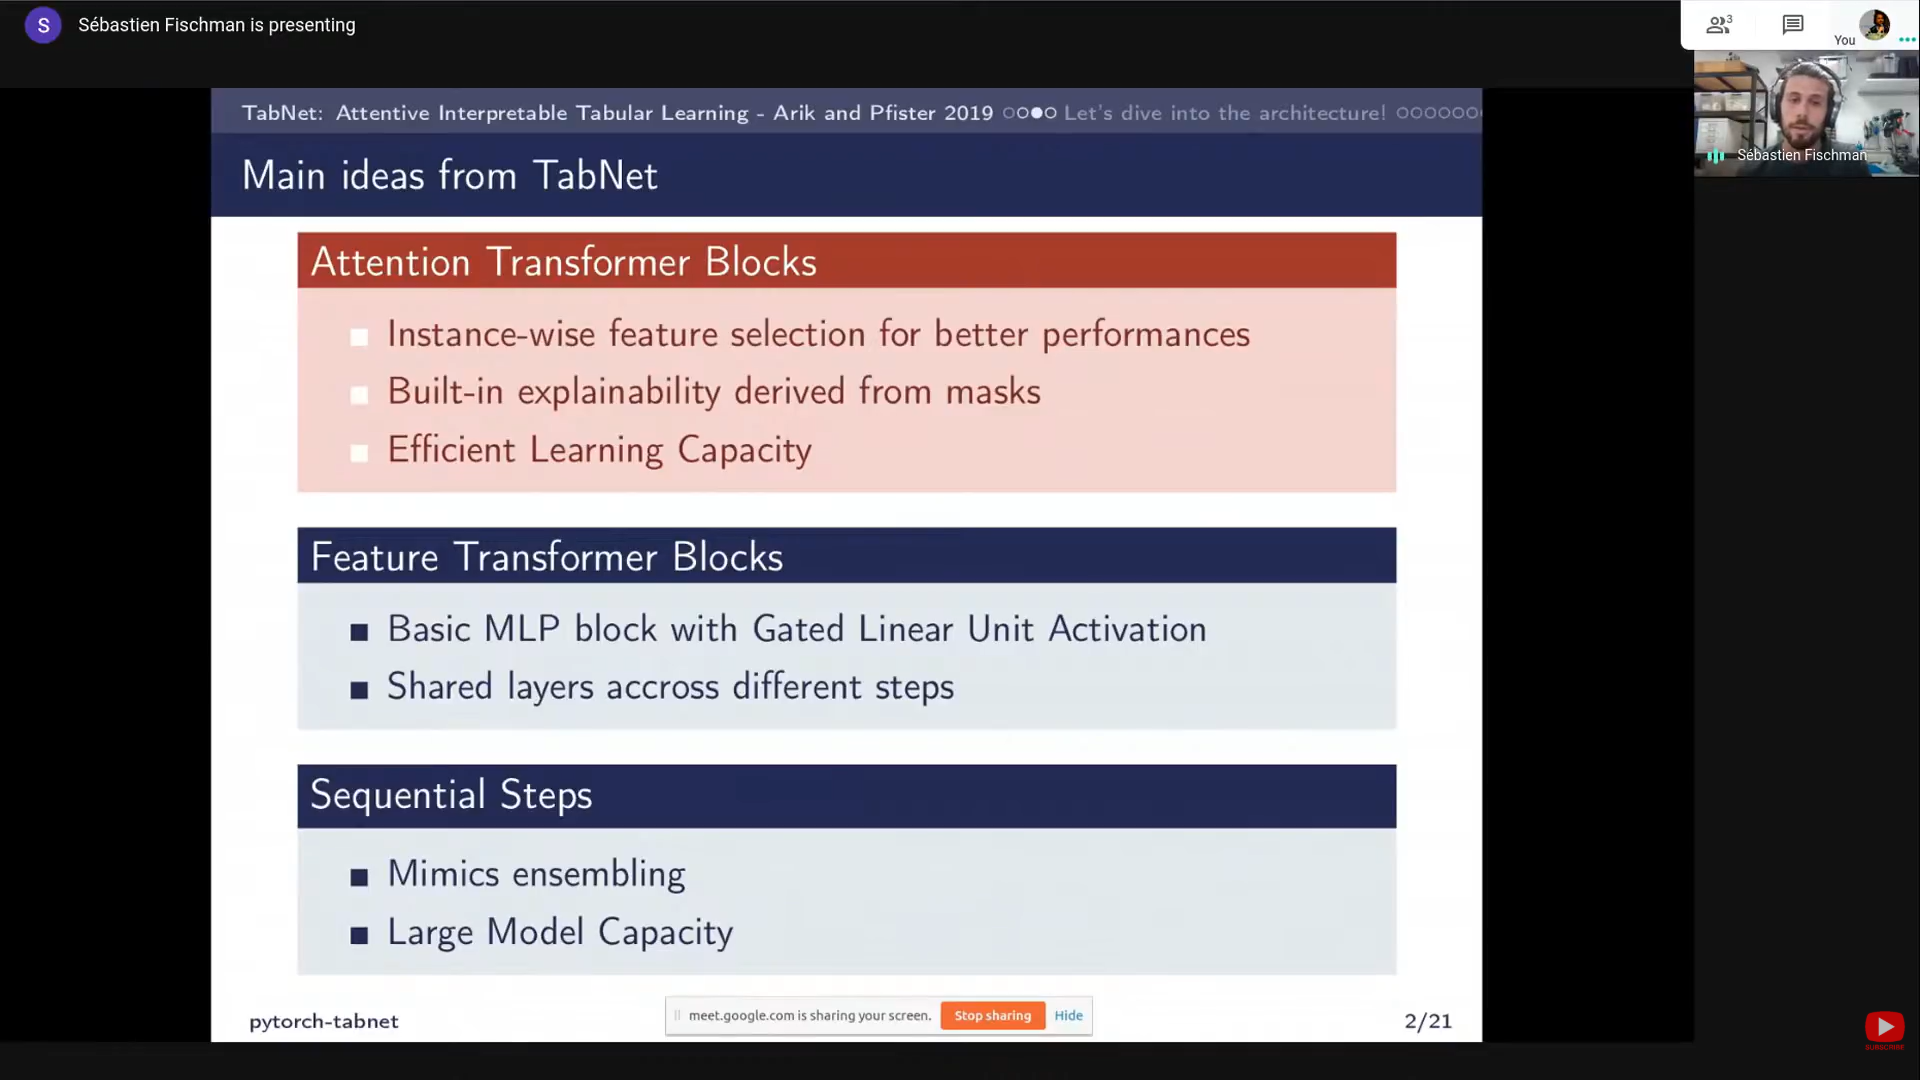
\includegraphics[width=1\linewidth]{TabNet的主要概念.png}
    \caption{TabNet的主要概念)}
    \label{fig:placeholder}
\end{figure}

\subsection{Global Architecture}
\begin{figure}[H]
    \centering
    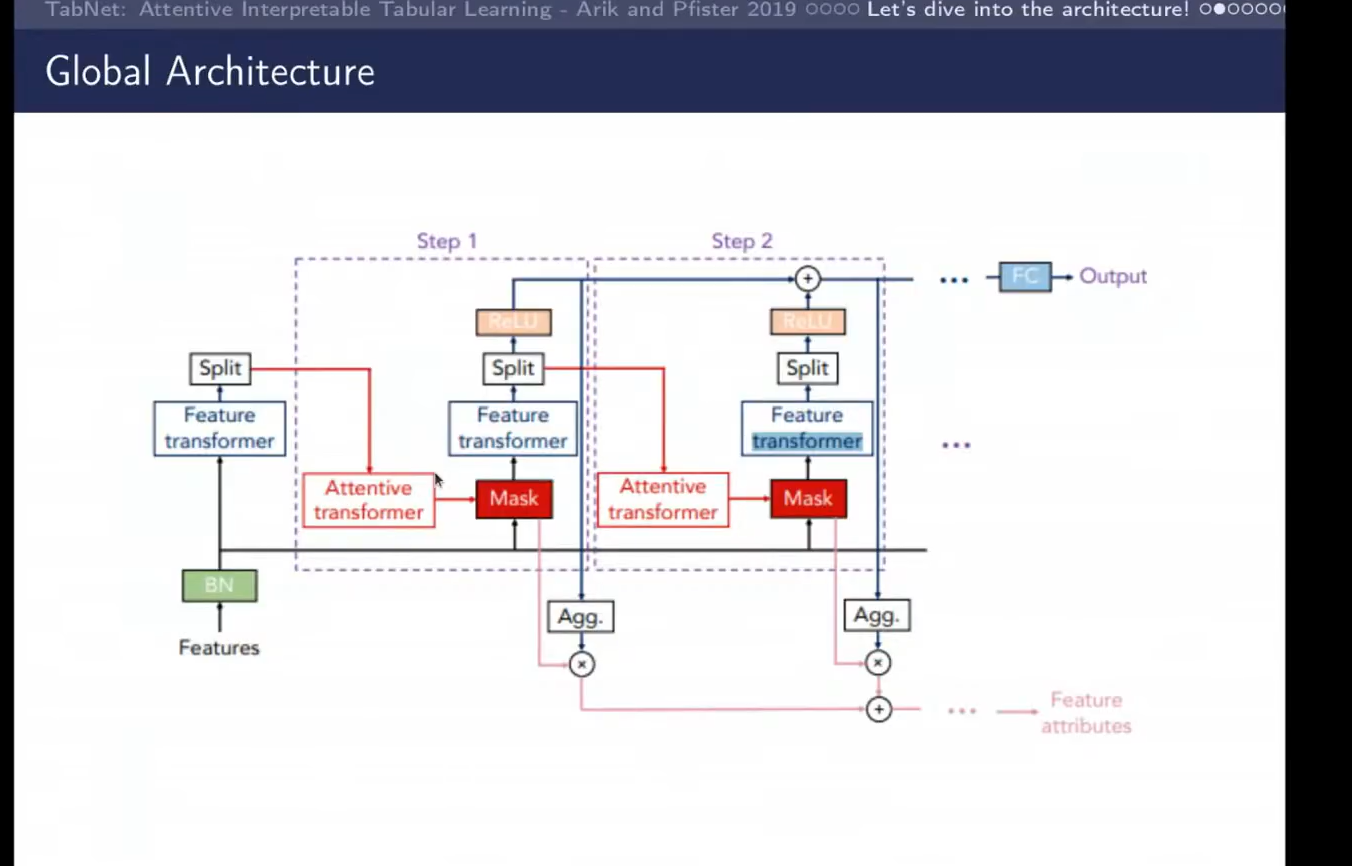
\includegraphics[width=1\linewidth]{TabNet的完整架構圖.png}
    \caption{TabNet的完整架構圖}
    \label{fig:placeholder}
\end{figure}

一開始原始資料在輸入時(Features)會先經過\textbf{Batch Normalization(BN)}，確保數據分布穩定，接著經過\textbf{Feature Transformer}和\textbf{split}後，進行單一步驟的運算處理(step1, step2)在每一個運算處理中，\textbf{Attentive Transformer}會根據前一步驟處理完的資訊，決定當前要看哪些特徵。再使用\textbf{Mask(遮罩)}作用於原始特徵上，去過濾掉不重要的資訊。 後續，\textbf{Feature Transformer}負責處理被 Mask 選中的特徵，提取深層的非線性關係。最後透過split分成兩條路，一路往上傳遞，作為該步驟對最終預測的貢獻；另一路傳往右邊，作為下一個步驟（Attentive Transformer）的參考資訊。值得注意的是，每個step的Masdk資訊會經過\textbf{Agg.(Aggregation)}處理並累加，這為模型提供了\textbf{可解釋性}的基礎。

\subsubsection{Feature Transformer}
\begin{figure}[H]
    \centering
    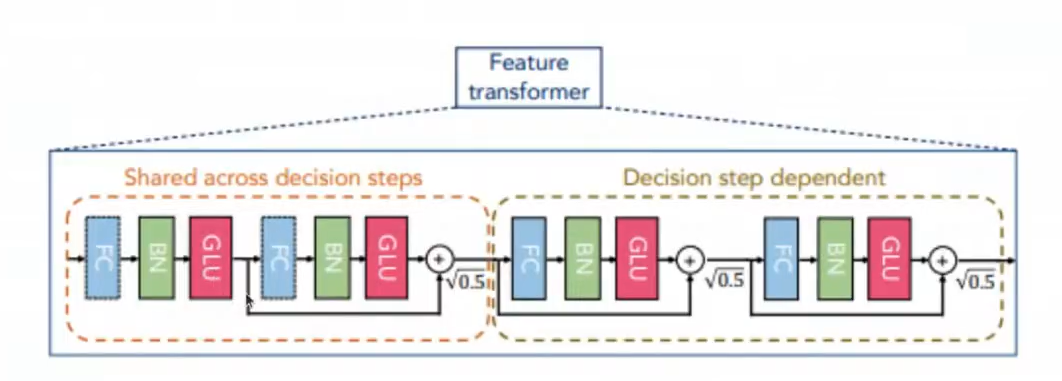
\includegraphics[width=1\linewidth]{TabNetFeatureTransformer.png}
    \caption{TabNet Feature Transformer}
    \label{fig:placeholder}
\end{figure}
由多個GLU blocks組成，以上圖為例來解釋。GLU blocks內部含有三個子套件：
\begin{itemize}
    \item Fully connect(FC)：神經網路中神經元的結構，進行基本的線性轉換(如：$y=Wx+b$)
    \item Batch Norm(BN)：將一小批標準化(Mini-batch)的平均值調整為0，標準差調整為1。
    \item Gated Linear Unit(GLU)：類似於門閥的功能，決定讓多少 x 的資訊通過，數學式： $GLU(x) = \sigma(x) \odot x $
\end{itemize}
其中GLU blocks間又有兩種關係：
\begin{itemize}
    \item Shared across decision steps：區塊在所有步驟中是共享參數的
    \item Decision step dependent：區塊是各步驟獨立
\end{itemize}
而每個獨立的區塊都有箭頭繞過處理層直接相加，這稱為Skip Connection，並乘以 $\sqrt{0.5}$ 來維持變數穩定。 \\
經過整串 Feature transformer後，Input size = $n_{features}$，Output size = $n_d + n_a$，這兩者分別為\textbf{Decision Dimension}和\textbf{Attention Dimension}

\subsubsection{Attentive Transformer}
一開始一樣會經過FC以及BN，此時的Input size是 $n_a$，接著會進行兩項重要的工程。
\begin{itemize}
    \item Prior Scales:用以紀錄看過哪些特徵，為了避免模型在每個步驟都重複看同樣的資訊。 \\
    (1) $P_0 = 1$：在第一步時，所有特徵都是平等的，沒有偏好。 \\
    (2) $P_i = \prod^{i}_{j=1}(\gamma - M_j)$：其中 $M_j$是之前步驟產生的Mask；$\gamma$(Relaxation factor)是一個\textbf{超參數}(通常大於1)，會強制模型去關注其他變數。
    \item SparseMax：用於特徵選擇，相較於Softmax而言，可以將特徵權重真的壓至0，能真的實現Instance-wise Selection(單一特徵選擇)；以及歸一化，指得是非零權重相加結果依然等於1，$\sum^{n}_{i=1}sparsermax(x)_i = 1, \forall x \in \mathbb{R}^n$。
    \item (補充)$Softmax = \frac{e^{z_i}}{\sum e^{z_j}}$
\end{itemize}
兩項工程結束後，output size = $n_{feature}$

\subsubsection{Self Supervised Learning}
屬於較新的內容，主要的概念在於透過預測隨機的masked features進行預訓練(pretrain)，適合用於少量的資料。

\begin{tcolorbox}
筆記作者：TRex \\ 
參考資料：\href{https://www.youtube.com/live/ysBaZO8YmX8?si=Esm2Al5lFKWaihMh}{\textbf{Pytorch-tabnet : Beating XGBoost on tabular data with deep learning}} \\ 
資料作者： \textbf{Sebastien Fischman}
\end{tcolorbox}

\end{document} 
